%!TEX root = ../nwoods_thesis.tex

\chapter{Simulation}\label{ch:simulation}

Comparing data collected by CMS to theoretical predictions is a complex task.
The theories described in Chapter~\ref{ch:SM} are understood in great detail, but using this knowledge to calculate observables is a nontrivial enterprise.
Once calculated, observables must be compared to data from a detector with finite resolution and subject to a number of experimental effects that do not exist in the rarefied world of quantum field theory.
The general strategy is to employ numerical simulations of individual collision events that involve a physics process of interest, and apply accurate simulations of the detector's response to these events to obtain samples that are directly comparable to data.
The success of all steps in this process at a high-luminosity hadron collider is one of the triumphs of the LHC era, with many observables in interesting processes simulated accurately to the level of a few percent.



\section{Monte Carlo Event Generation}

Even in trivial cases, it would be impossible to integrate over the phase space of hard scattering outcomes determined from theory, convolved with matter interactions, detector effects, and other experimental factors, to calculate observables analytically.
Particle interactions are well-understood on a microscopic scale, but it is extremely difficult to extrapolate from this first-principles understanding to a description of the macroscopic behavior of an ensemble of particles as needed to make predictions about fundamentally stochastic processes.
Observable spectra are therefore modeled with the Monte Carlo (MC) method~\cite{Metropolis:10.2307.2280232,Olive:2016xmw}, a numerical integration technique so named because, like a casino, it relies heavily on random numbers\footnote{Pseudorandom numbers are actually used, but there is no difference in practice as long as a good pseudorandom number generator (PRNG) is chosen and seeded properly. The Mersenne Twister algorithm~\cite{Matsumoto:1998:MTE:272991.272995} is the modern standard among general-purpose PRNGs in physics and elsewhere.}.
The scattering amplitudes for a process are calculated from theory at a chosen perturbative order, and for each simulated event a configuration of final state particles is selected at random from this phase space.
The final state particles are propagated through decays, radiation, hadronization, and interaction with other matter---such as the detector---based on well-understood physics principles, and the outcome of any stochastic process is chosen at random from a realistic set or distribution of possibilities.
In the limit of a large number of simulated events, the distributions from the simulated detector will converge to be directly comparable to aggregated data.
Individual steps in this process are detailed in the following sections.


\subsection{Matrix Element and Hard Process Generation}

Event generator programs start by calculating the scattering amplitudes for a process at a chosen order in perturbation theory.
For example, the generator {\MGAMC}~\cite{Alwall:2014hca} generates all the relevant Feynman diagrams up to NLO and calculates the matrix elements for them.
Others, like {\POWHEG}~\cite{Nason:2004rx,Frixione:2007vw,Alioli:2010xd}, {\SHERPA}~\cite{Gleisberg:2008ta} and {\MCFM}~\cite{Campbell:1999ah,Campbell:2011bn,Campbell:2015qma}, are not fully general but have a broad range of physics processes implemented at NLO\@; {\SHERPA} and {\MCFM} can do some calculations at NNLO~\cite{Boughezal:2016wmq}.
Events are generated across the entire allowed phase space, either uniformly or with the specific distribution dictated by one of several ``importance sampling'' techniques~\cite{Lepage:1977sw,Olive:2016xmw} which ensure appropriate statistical coverage in regions where the distribution has a large slope or value.
Each event is assigned a weight $w \in (0,1)$ based on the scattering amplitude in that region of phase space and the probability of having an appropriate initial state based on the PDFs discussed in Section~\ref{sec:pp}.
The sample is then ``unweighted'' to a subset that is directly comparable to data by removing events with a probability proportional to $1 - w$.


\subsection{Parton Shower, Hadronization, and Underlying Event}\label{sec:partonShower}

Processes generated above leading order may have extra radiation, as in the real emission diagrams of Fig.~\ref{fig:zzNLO}.
In the case of calculations at higher orders in QCD, the emissions are quarks and gluons which fragment, hadronize, decay, etc.
This process is handled by a parton shower (PS) MC program such as {\PYTHIA}~8~\cite{Sjostrand:2014zea} (used for most simulations used in this analysis), \textsc{Herwig}~\cite{Bahr:2008pv,Bellm:2015jjp}, or {\SHERPA}~\cite{Gleisberg:2008ta}.
In {\PYTHIA}, parton showering is simulated with the Lund string model~\cite{Andersson:1978vj,Andersson:1983jt, Andersson:2001yu,Olive:2016xmw}, which treats gluons as ropes connecting color charged particles whose tension increases as the quarks move apart.
When a rope stretches too far, it breaks, producing a quark pair at the new rope ends.

Parton shower programs also handle radiation of soft gluons from color charged particles and photons from electrically charged particles~\cite{Sjostrand:2004ef}.
The emitter may be an incoming parton (initial state radiation, ISR), a virtual particle exchanged during the interaction, or an outgoing particle (final state radiation, FSR).
The distinction between ``soft'' radiation that should be handled by the PSMC and ``hard'' emission present in the matrix element is not well defined, so it is important to avoid double-counting regions of phase space at the boundary between the processes.
This is done with jet matching~\cite{Alwall:2014hca,Olive:2016xmw}.
At tree level, matching may be achieved by enforcing a jet energy cutoff: partons from the matrix element must have energy $E > E_\text{cut}$, and the PSMC is responsible for any softer radiation.
At NLO, loop diagrams carry divergences that must be canceled by divergences of opposite sign in the infrared radiation regime, which the cutoff would prevent, so a more sophisticated scheme must be used which weights some events negatively to handle destructive interference~\cite{Alwall:2014hca} or modifies the shower development algorithm~\cite{Nason:2004rx,Frixione:2007vw}.

When combining showered samples that have different jet multiplicities at hard process level the task becomes even more difficult because the phase space of events with $n$ jets in the matrix element that gain another from the PS overlaps with the phase space of events with $n+1$ jets at matrix element level.
This problem can be solved with one of several jet merging algorithms~\cite{Alwall:2007fs,Alwall:2008qv,Alwall:2014hca,Rauch:2016pai}.
The MLM~\cite{Mangano:2006rw} and CKKW~\cite{Catani:2001cc} algorithms implement merging for tree-level diagrams of different jet multiplicities by cutting (MLM) or weighting (CKKW) events based on the probability that such an event would originate from the matrix element or PS\@.
The FxFx algorithm implements merging when one-loop diagrams are included~\cite{Frederix:2012ps}.

PSMC programs provide several more features that are vital in obtaining a faithful reproduction of data, especially in events with only soft hadronic activity.
The radiation described above affects the {\pt} of the hard scatter system, so PSMCs must ``retroactively'' adjust the kinematics generated by the matrix element MC\@.
The underlying event, further QCD interactions that happen below the regime that can be calculated perturbatively, are modeled phenominologically~\cite{Olive:2016xmw,Sjostrand:2014zea}.
This includes soft color exchange between fragments of the colliding hadrons that sends proton remnants into the detector in the form of extra soft hadrons~\cite{Sjostrand:2004pf}.
There is also a possibility that multiple pairs of partons will undergo hard interactions in the same proton-proton collision, essentially combining two quasi-independent hard scatters~\cite{Sjostrand:2004ef,Manohar:2012jr}.


\subsection{Pileup Simulation}

The high per-bunch luminosity of the LHC causes multiple collisions to occur in each bunch crossing.
The extra interactions are called pileup.
To account for this effect, CMS simulations include extra minimum-bias collision events overlaid on top of the primary collision~\cite{Banerjee:1742-6596-396-2-022003, Hildreth:1742-6596-664-7-072022}.
This includes simulated pileup interactions that are time evolved to reproduce the effects of ``out-of-time'' pileup from previous bunch crossings.
Because MC samples are produced before the pileup profile can be measured in data, simulated events are reweighted based on the number of pileup interactions such that the distribution of the number of reconstructed vertices becomes similar to that in data.


\subsection{Samples Used in this Analysis}\label{sec:samples}

The $\qqb \to \ZZ$, $\Pq\Pg \to \ZZ$, $\Pg\Pg \to \PH \to \ZZ^\ast$, and $\qqb \to \PZ \to 4\ell$ samples are produced at NLO with {\POWHEG}~\cite{Alioli:2008gx,Nason:2004rx,Frixione:2007vw,Alioli:2010xd, Melia:2011tj} and scaled to the NNLO total cross section with $K$~factors of 1.7 for the Higgs sample and 1.1 for the others~\cite{Cascioli:2014yka}.
The non-Higgs {\POWHEG} samples include {\ZZ}, {\Zgs}, and $\Pa^\ast\Pa^\ast$ production with a generator-level constraint of $m_{\ell\ell'} > 4\GeV$ for all opposite-charge lepton pairs, to limit the generated phase space to only regions of interest and far from infrared divergences.
For the inclusive cross sections and differential cross sections in fully leptonic observables, this {\POWHEG} sample is considered the primary theory prediction.
For the differential cross sections in jet-related variables, {\MGAMC} is used for the nominal sample, because it has an extra jet at matrix-element level, merged with the PS jets using the FxFx scheme.
Box diagram $\Pg\Pg \to \ZZ$ samples are generated with {\MCFM} at LO~\cite{Campbell:2010ff}; these are scaled to NLO with a $K$~factor of 1.7~\cite{Caola:2015psa}.

Background {\WZ} events are produced with {\POWHEG} with the same settings as the {\ZZ} sample while {\TTZ} and {\WWZ} samples are generated at LO with {\MGAMC}.
Electroweak and non-VBS {\ZZjj} samples are produced with {\MGAMC} for the VBS and aQGC searches and with {\PHANTOM} for the cross section measurements~\cite{Ballestrero:2007xq}.
Samples with nonzero aTGCs are generated at LO with {\SHERPA}~\cite{Gleisberg:2008ta} and scaled such that the total yield from the SM {\SHERPA} sample is the same as the yield from the {\POWHEG} {\ZZ} sample.
Signal samples for the aQGC search are made with {\MGAMC}.

All samples use the NNPDF3.0 PDF sets~\cite{Ball:2014uwa}.
Parton showing, hadronization, and underlying event simulation are done with {\PYTHIA} using the CUETP8M1 tune~\cite{Khachatryan:2015pea} for all samples except the aTGC samples, for which {\SHERPA} performs these tasks.


\section{Detector Simulation}

To incorporate experimental effects into MC samples, the detector and the final state particles' interactions with it are simulated with the highest possible level of detail~\cite{Banerjee:1742-6596-396-2-022003, Hildreth:1742-6596-664-7-072022}.
The detector geometry and material, including both instrumented and non-instrumented components, are modeled with the {\GEANTfour} package~\cite{Agostinelli:2002hh}, which describes microscopic particle interactions with matter over a wide range of energies and propagates the effects of these interactions to their macroscopic consequences.
Stochastic effects are again implemented with Monte Carlo methods that select outcomes at random from realistic distributions of possibilities.
The {\GEANTfour} simulation includes a detailed model of the magnetic field, so particle trajectories are calculated correctly, and the generation of secondary particles like {\epem} pairs from photons interacting with tracker material.
Charge deposition in silicon, scintillation in clear crystals, hadronic showers from nuclear interactions, and gas ionization are all included, among many other processes, so detector signals are derived from microscopic interactions too, and {\GEANTfour} has signal digitization capabilities which ensure that the signals coming out of the simulated detector are exactly those that would be produced by the real detector in the same situation.

The simulated signals are fed into the same reconstruction software as is used for data (see Chapter~\ref{ch:reco}).
The same analysis strategy may then be used for MC samples and data, and comparing the results is meaningful.
Though every effort is made to model the detector accurately, no simulation can incorporate all real effects with perfect fidelity.
Monte Carlo samples must be produced before data are actually collected, so the final detector alignment and calibration cannot be known exactly, and conditions may change mid-run if---for example---a subdetector channel goes dead or LHC beam conditions change.
Residual corrections for these small effects are applied to final physics objects in the final steps of the analysis to make distributions of interest, such as dilepton mass around the {\PZ} resonance or the overall jet {\pt} spectrum, match in aggregate.
The overall level of agreement between data and simulation may be seen in Fig.~\ref{fig:dataMCRatio}, which shows the invariant mass of {\epem} events around the {\PZ} resonance for simulated samples and data, and their ratio.

\begin{figure}[htbp]
  \begin{center}
    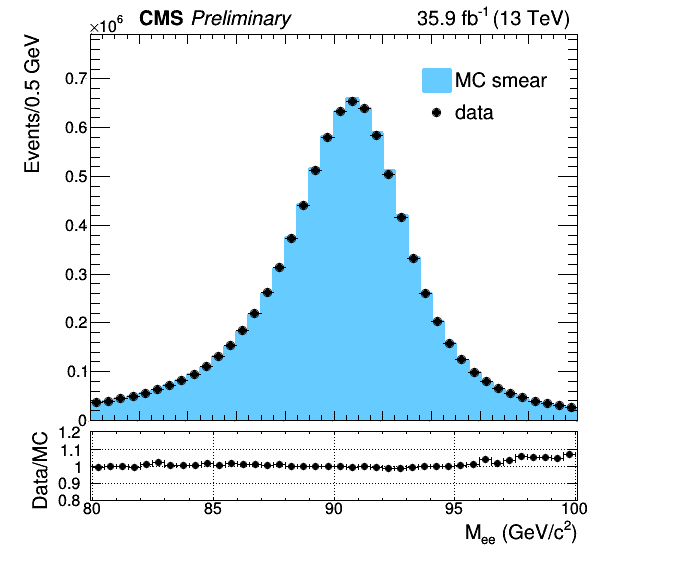
\includegraphics[width=0.48\textwidth]{simulation/EBEBInvMass2016.png}
    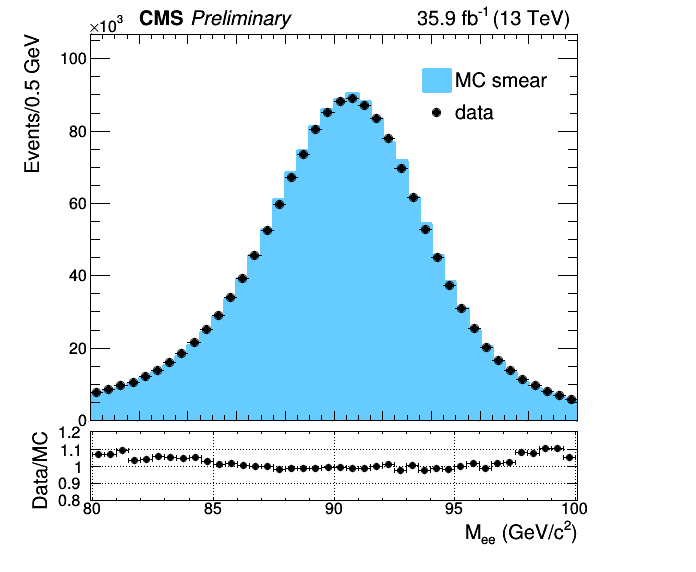
\includegraphics[width=0.48\textwidth]{simulation/EEEEInvMass2016.png}
    \caption[Comparison of data and simulation in {\epem} events around the {\PZ} resonance]{
        The invariant mass of {\epem} events with both electrons in the barrel (left) and both electrons in the endcaps (right) in the whole 2016 dataset after all corrections are applied.
        The lower plots show the ratio of data and simulation to show the level of agreement achieved.
      }\label{fig:dataMCRatio}
  \end{center}
\end{figure}
